\part{Introduction}
\begin{frame}
\partpage
\end{frame}

%\begin{frame}{Introduction: Outline}
%\small
%  \tableofcontents[subsectionstyle=hide]%[pausesections]
%\end{frame}

\begin{frame}{Health and Safety}
\begin{columns}[c]
\begin{column}{0.33\textwidth}
\begin{center}

\includegraphics[width=0.8\textwidth,height=0.5\textheight,keepaspectratio]{imgs/health-safety-1.png}\\

\includegraphics[width=0.8\textwidth,height=0.5\textheight,keepaspectratio]{imgs/health-safety-4.png}
\end{center}
\end{column}
\begin{column}{0.33\textwidth}
\begin{center}

\includegraphics[width=0.8\textwidth,height=0.5\textheight,keepaspectratio]{imgs/health-safety-2.png}\\
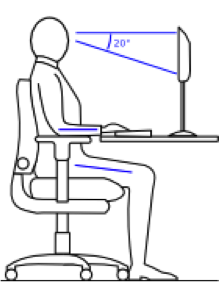
\includegraphics[width=0.8\textwidth,height=0.5\textheight,keepaspectratio]{imgs/health-safety-5.png}
\end{center}
\end{column}
\begin{column}{0.33\textwidth}
\begin{center}

\includegraphics[width=0.8\textwidth,height=0.5\textheight,keepaspectratio]{imgs/health-safety-3.png}\\

\includegraphics[width=0.8\textwidth,height=0.5\textheight,keepaspectratio]{imgs/health-safety-6.png}
\end{center}
\end{column}
\end{columns}
\end{frame}

\section{Who are we?}
\begin{frame}{UIS: Research and Institutional Services Division}
Your trainer for today will be:\\
\begin{itemize}
  \item Paul Sumption --- Research Computing Technical Liaison
  \item\alert{Please ask questions and let us know if you need assistance.}
\end{itemize}
\end{frame}

\section{Training Accounts}
\begin{frame}{Introduction: Training accounts}
\begin{itemize}
\item{\alert{For our practical exercise's we will use HPC training accounts.}}
\pause
\item{You will find a piece of paper on your desk.}
\pause
\item{1: Your training account details.}
\pause
\item{Your training account will only be valid for today.}
\end{itemize}
\end{frame}

\section{Login node for today}
\begin{frame}{Introduction: Login node}
\begin{itemize}
\item{\alert{For our practical exercise's we will use the login node: login-cpu.hpc.cam.ac.uk.}}
\pause
\item{Later in the course you will see that different nodes types may require you to use other login nodes.}
\end{itemize}
\end{frame}

\section{Security}
\begin{frame}{Introduction: Security}
\begin{itemize}
\item{\alert{Boring but very, very important${}\ldots$}}
\pause
\item{Cambridge IT is under constant attack by would-be intruders.}
\pause
\item{Your data and research career is threatened by intruders.}
\pause
\item{\alert{Cambridge systems} are high profile and popular targets.}
\pause
\item{\alert{Don't let intruders in.}}
\end{itemize}
\end{frame}

\begin{frame}{Introduction: Security}
\begin{enumerate}
\item{\alert{Keep your password (or private key passphrase) safe.}}
\pause
\item{\alert{Always choose strong passwords.}}
\pause
\item{\alert{Your UIS password is used for multiple systems so keep it secure!}}
\pause
\item{Keep the software on your laptops/tablets/PCs up to date this includes home computers especially if you are using the VPN to connect in.}
\pause
\item{Don't share accounts (this is against the rules anyway).}
\end{enumerate}
\end{frame}

\section{Introduction: Pre-requisites}
\begin{frame}{Pre-requisites}
\begin{itemize}
\item{Pre-requisites: Basic Unix/Linux command line experience}
\pause
\item{Suggested Courses:}
\item Unix: Introduction to the Command Line Interface (Self-paced)
\small {\url{https://www.training.cam.ac.uk/ucs/Course/ucs-unixintro1}} 
\pause
\item Shell scripting experience is desirable:
\item Unix: Simple Shell Scripting for Scientists
\small {\url{https://www.training.cam.ac.uk/ucs/Course/ucs-scriptsci}} 
\end{itemize}
\end{frame}

\subsection{Navigating the command line }
\begin{frame}{Navigating your terminal}
Useful commands for navigating your terminal.
\begin{itemize}
\item{\alert{\footnotesize cd \textless dirname\textgreater } - change into a directory }
\item{\alert{\footnotesize ls \textless dirname\textgreater } - list the contents of a directory}
\item{\alert{\footnotesize cd or cd \path{~}} - change into your home folder}
\item{\alert{\footnotesize cd .. } - change back one folder}
\item{\alert{\footnotesize man ls } - will bring up the manual page for the ls command}
\item{\alert{\footnotesize pwd } - print working directory}
\end{itemize}
\end{frame}
